% ================= PART I =================
\part{Introduction to GLMs}

\chapter{OLS}

\Exploration

At this point in the chapter I approach OLS as a total beginner trying to explore the concept of Ordinary Least Squares. To start, the best way to approach any exploration of new concepts is to research using YouTube University, so I searched ``OLS'' on YouTube and got this.

\begin{screenshot}

\includegraphics[width=\linewidth]{assets/exploration-youtube-ols.png}
\end{screenshot}
\captionof{figure}{OLS video from YouTube \citep{sds2023}.}
\explorationsource{Super Data Science (2023), \textit{Introduction to Ordinary Least Squares with Examples}, YouTube.}

\vspace{6pt}
So what is ``Ordinary Least Squares''?

This image is a practical example of OLS (linear regression) showing the line of best fit, model accuracy, and sum of squares (minimised).

\begin{screenshot}
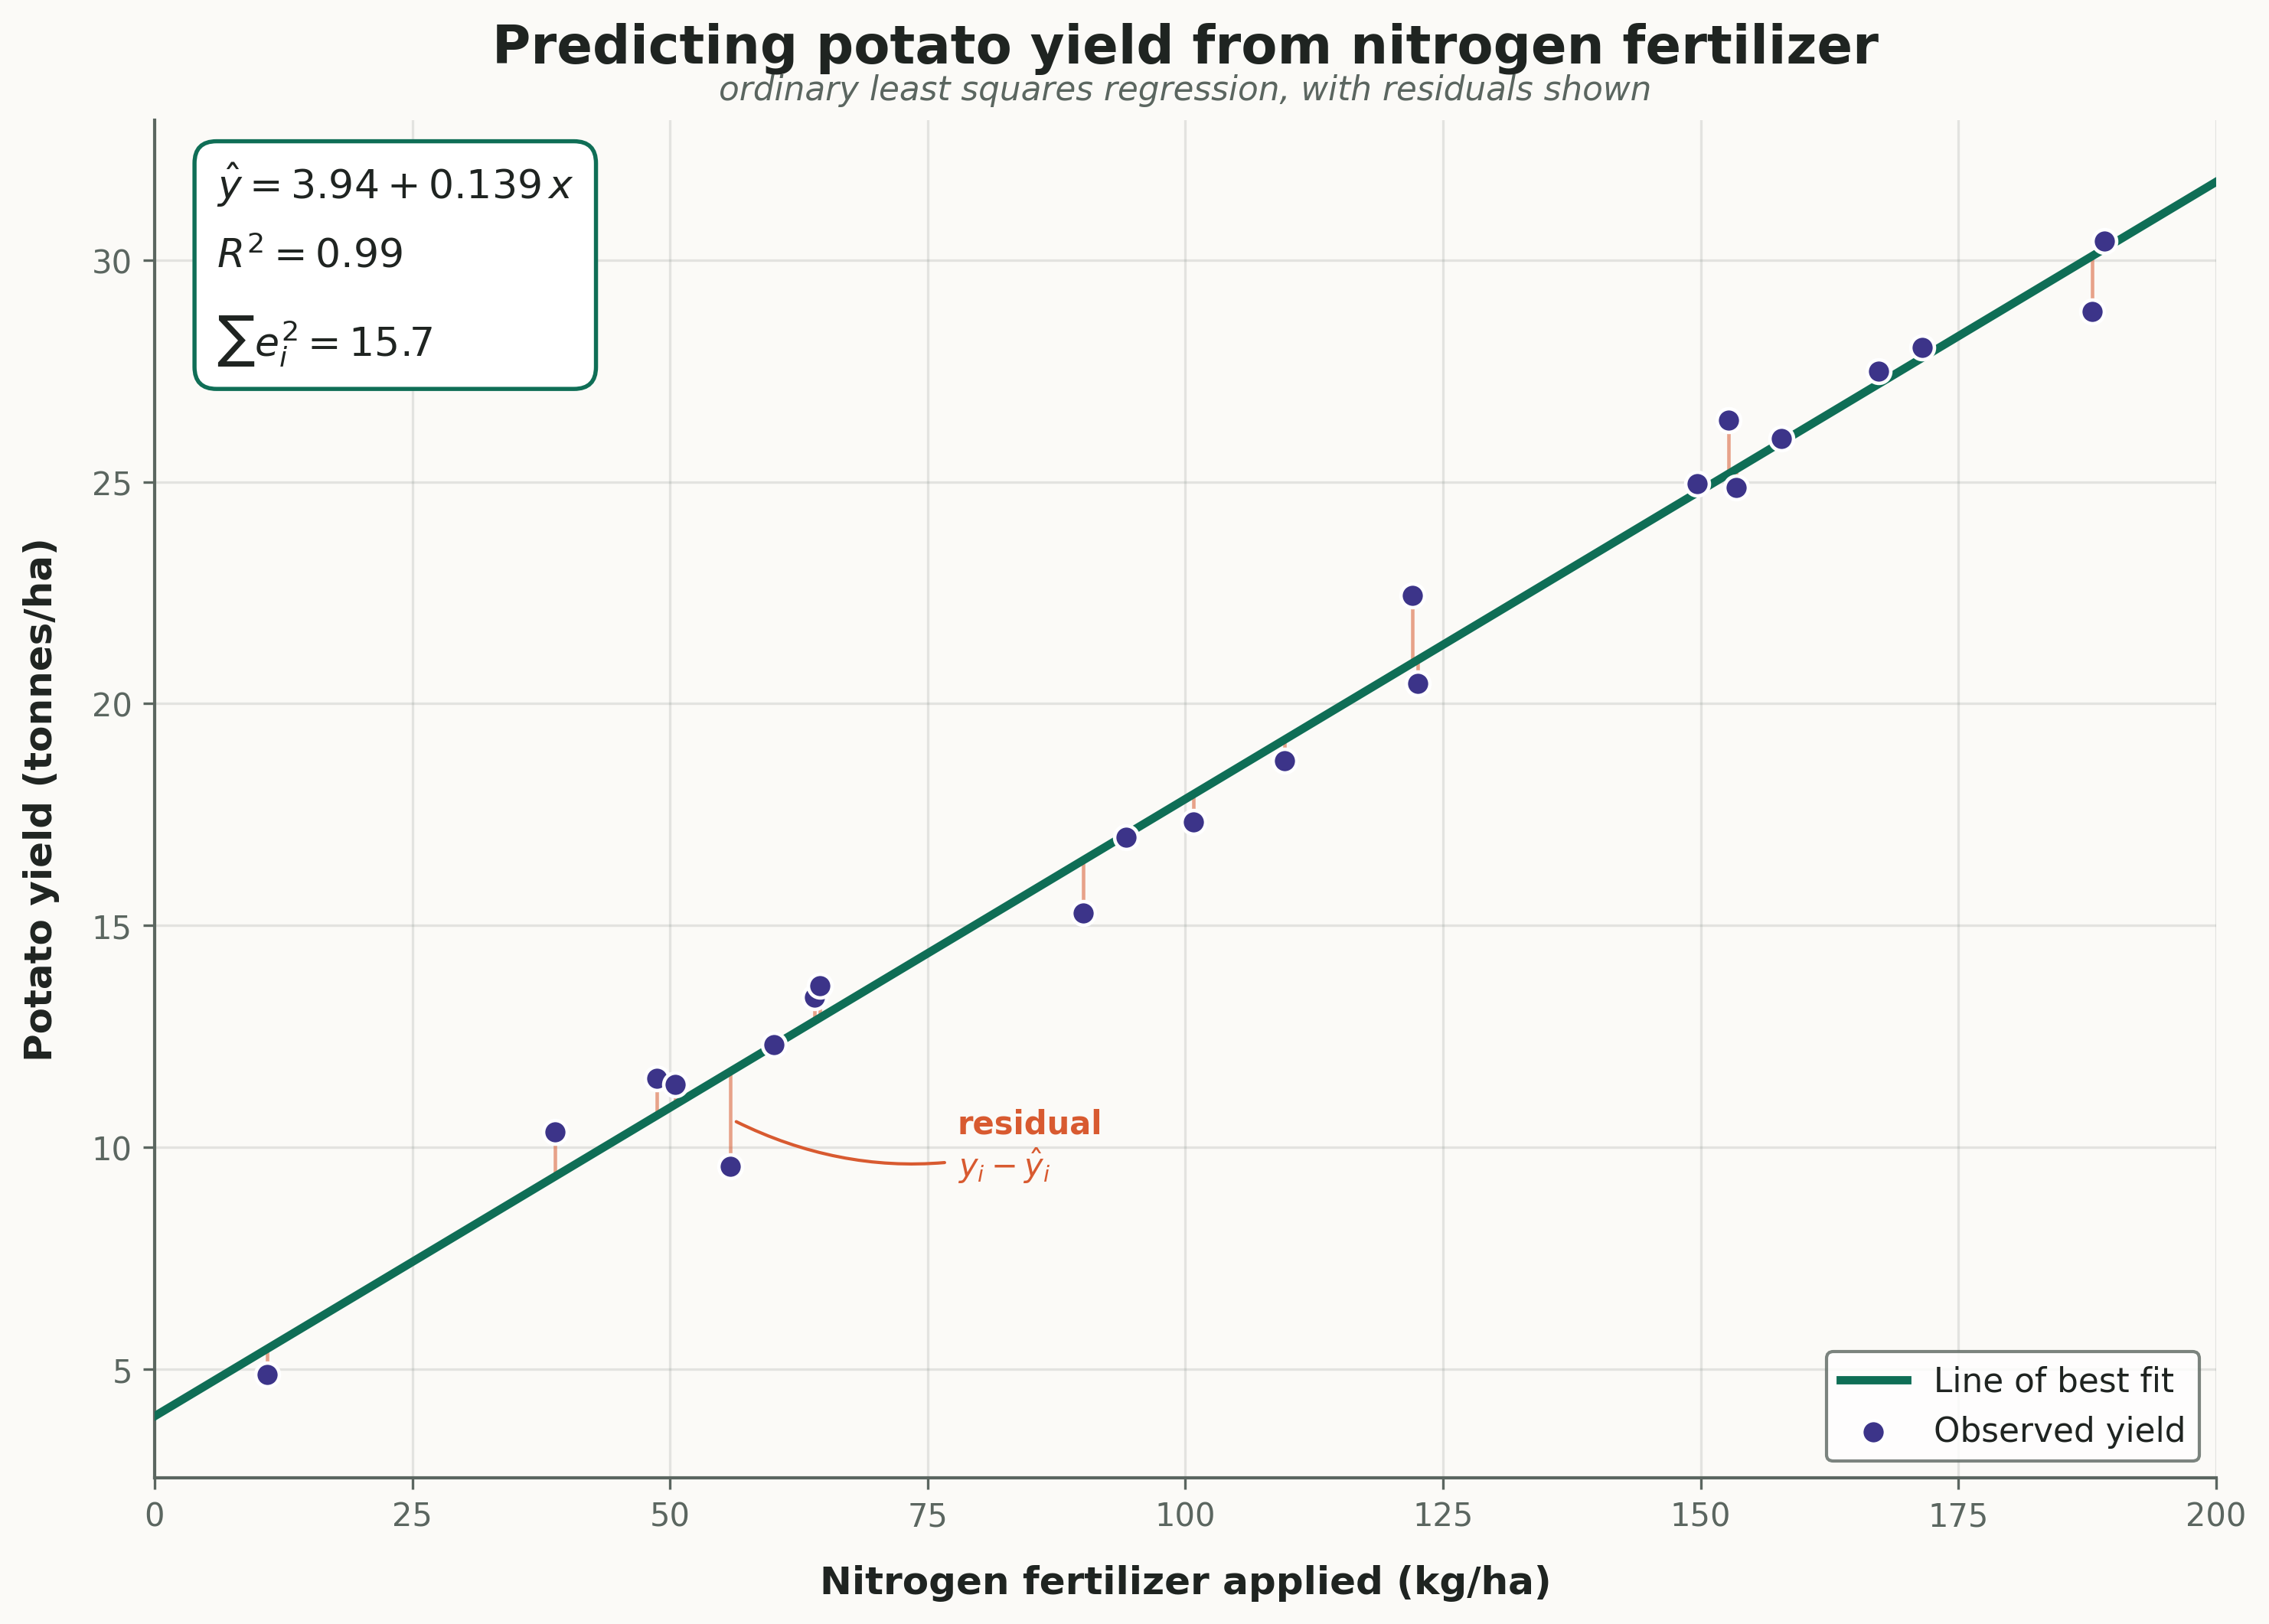
\includegraphics[width=0.85\linewidth]{assets/exploration-ols-example.png}
\end{screenshot}
\captionof{figure}{A practical example of OLS (linear regression): the line of best fit, model accuracy, and the (minimised) sum of squares.}

We move further to the Cognition phase, where things get more formal and definitions and some fun maths appear.

\Cognition

\subsection*{Linear Regression}
A model used in statistics to assess the connection between a scalar response (dependent variable) and one or more explanatory factors (independent variables or regressors) is called linear regression.
\begin{mathbox}
\[
y_i = \beta_0 + \beta_1 x_i + \epsilon_i
\]
\end{mathbox}

\subsection*{Simple Linear Regression}
A linear regression with just one explanatory variable. It is a clear system with no confounding, where cause is most likely linked directly to effect.

\subsection*{Multiple Linear Regression}
A linear regression with two or more explanatory variables. It is more interesting and more prone to confounding, since cause doesn't always mean effect; it could be a combination of causes, or a cause could appear prominent only because of another variable.

To see why the exponential family occupies such a central place in GLM theory, it helps to start with the simple linear model.

\subsection*{The Linear Model as a Starting Point}
The simple linear model is written
\begin{mathbox}
\[
Y_i = \beta_0 + \beta_1 x_i + \epsilon_i
\]
\end{mathbox}
where $\epsilon_i$ is an error term assumed to be normally distributed with mean 0 and constant variance $\sigma^2$, that is $\epsilon_i \sim N(0,\sigma^2)$. Because $Y_i$ is a constant $(\beta_0+\beta_1 x_i)$ plus a normally distributed random variable, $Y_i$ itself is normally distributed:
\begin{mathbox}
\[
Y_i \sim N(\mu_i,\sigma^2), \qquad \mu_i = \beta_0 + \beta_1 x_i
\]
\end{mathbox}

In other words, the linear combination of the explanatory variable and its coefficient does not directly define $Y_i$, it defines where the mean of $Y_i$ sits. The error term provides the randomness and its distributional form, while the linear predictor $\beta_0+\beta_1 x_i$ simply drags that mean to where the covariate $x_i$ indicates it should be. This separation, a distributional assumption on one side and a linear predictor governing the mean on the other, is precisely what GLMs later generalise.

\subsection*{Extending to Multiple Explanatory Variables and Vector Responses}
The same logic extends naturally once there is more than one explanatory variable. Instead of a single $x_i$, we have a row of covariates for each observation, and the mean becomes
\begin{mathbox}
\[
\mu_i = \beta_0 + \beta_1 x_{i1} + \beta_2 x_{i2} + \cdots + \beta_p x_{ip} = x_i^\top \beta
\]
\end{mathbox}
with $Y_i \sim N(\mu_i,\sigma^2)$ still holding, only now $\mu_i$ is a linear combination of several predictors rather than one. Written for the whole sample at once, this is $Y = X\beta + \epsilon$, with $X$ the design matrix and $\beta$ the vector of coefficients.

\subsection*{Where the Linear Model Falls Short}
The assumptions underpinning the linear model, constant variance, a normally distributed response, and a mean that varies linearly with the predictors, do not hold for a great deal of real data. Counts of events, binary outcomes (success/failure), and proportions are common, none of which are well described by a normal distribution with constant variance. A count cannot be negative, and its variance tends to grow with its mean; a binary outcome only takes two values; a proportion is bounded between 0 and 1.

There is also the question of the relationship between the response mean and the linear predictor. In the classical linear model that relationship is direct: $\mu_i$ literally equals the linear combination of covariates. But for many response types above, a straight linear relationship on the original scale does not make sense; for a binary outcome, what varies linearly with the covariates is more naturally the log-odds of success (the logit) rather than the probability itself.

Historically, fitting anything outside the normal linear model was difficult because closed-form estimators generally do not exist once the response distribution departs from normality or the mean is connected to the predictors through a nonlinear transformation. Iterative fitting procedures, developed to extend maximum likelihood estimation into settings without closed-form solutions, changed this: estimation still proceeds via an iteratively reweighted least-squares computation, echoing the linear model even as the distributional assumptions underlying it change entirely.

\subsection*{Deriving the Normal Equations by Hand}
For simple linear regression, we are fitting $\hat y_i = \beta_0+\beta_1 x_i$, with residual $e_i = y_i - \hat y_i$. Residuals are not summed directly, since positive and negative errors would cancel; instead the sum of squared residuals is minimised,
\begin{mathbox}
\[
S(\beta_0,\beta_1) = \sum_{i=1}^n \left(y_i - \beta_0 - \beta_1 x_i\right)^2
\]
\end{mathbox}

\begin{theorem}[Normal Equations]
Differentiating $S(\beta_0,\beta_1)$ with respect to each parameter and setting both to zero gives the normal equations \citep{dobson2018,casella2002}:
\begin{mathbox}
\[
\frac{\partial S}{\partial \beta_0} = -2\sum_{i=1}^n \left(y_i-\beta_0-\beta_1 x_i\right) = 0, \qquad
\frac{\partial S}{\partial \beta_1} = -2\sum_{i=1}^n x_i\left(y_i-\beta_0-\beta_1 x_i\right) = 0
\]
\end{mathbox}
Expanding the first and solving for $\beta_0$ gives $\beta_0 = \bar y - \beta_1\bar x$, which also shows the fitted line always passes through $(\bar x,\bar y)$. Substituting this into the second equation and simplifying gives the slope,
\begin{mathbox}
\[
\beta_1 = \frac{\sum_{i=1}^n (x_i-\bar x)(y_i-\bar y)}{\sum_{i=1}^n (x_i-\bar x)^2}
\]
\end{mathbox}
the covariance of $x$ and $y$ divided by the variance of $x$. Because $S(\beta_0,\beta_1)$ is a sum of squares, it is convex, so the second-order conditions are automatically satisfied and this stationary point is guaranteed to be a minimum.
\end{theorem}

\subsection*{Matrix Form of OLS}
The scalar derivation generalises directly to any number of predictors. Stacking the data gives $Y = X\beta+\epsilon$, with fitted values $\hat Y = X\beta$ and residual vector $e=Y-X\beta$. The sum of squared residuals is
\begin{mathbox}
\[
S(\beta) = e^\top e = (Y-X\beta)^\top(Y-X\beta) = Y^\top Y - 2\beta^\top X^\top Y + \beta^\top X^\top X \beta
\]
\end{mathbox}
Differentiating with respect to $\beta$ using the standard identities $\partial(\beta^\top X^\top Y)/\partial\beta = X^\top Y$ and $\partial(\beta^\top X^\top X\beta)/\partial\beta = 2X^\top X\beta$ \citep{casella2002}, and setting the result to zero, gives the normal equations in matrix form, $X^\top X\beta = X^\top Y$. Provided $X^\top X$ is invertible,
\begin{mathbox}
\[
\hat\beta = (X^\top X)^{-1}X^\top Y
\]
\end{mathbox}
which is exactly the closed-form estimator introduced as a term in Chapter 3, now derived rather than quoted. The Hessian $2X^\top X$ is positive semi-definite by construction, confirming this stationary point is a minimum \citep{dobson2018}. Rearranging $X^\top X\hat\beta = X^\top Y$ also gives $X^\top(Y-X\hat\beta)=0$, i.e.\ $X^\top e = 0$: the residual vector is orthogonal to every column of $X$, the orthogonality condition referenced under the Transposed Matrix term.

\Reflection

Looking back on the process of learning Ordinary Least Squares, I can say with confidence that I now understand both the intuition behind it and the mathematics underpinning it. Two questions arose along the way and were already answered, in passing, during the Cognition phase. Naming a question clearly is often what turns a passively absorbed derivation into a properly internalised one.

\begin{questionbox}[: Why do we need models at all?]
A model is a representation of a real-world process, constructed so that inferences can be made about the future behaviour of that process without repeating the underlying experiment every time. An experiment cannot be run on a future outcome, since that outcome does not yet exist empirically; data collection is also costly, so it would be far from optimal to repeat an experiment in full each time a new inference is required. The most intuitive model of all is a straight line, the line of best fit, from which it becomes possible both to predict future outcomes and to quantify how wrong those predictions are likely to be.
\end{questionbox}

\begin{questionbox}[: Why are the residuals squared before being summed?]
Each residual measures how wrong a single prediction is, and each residual carries a sign. Summing the residuals directly would allow positive and negative errors to cancel, leaving only the net direction in which predictions err rather than their overall magnitude. Squaring removes the sign while preserving, and emphasising, the size of the deviation. The resulting sum of squared errors is the quantity Ordinary Least Squares minimises.
\end{questionbox}

\Application

To put the theory into practice, a dataset was simulated in R to echo the exploration-phase example: nitrogen fertilizer applied (kg/ha) as the predictor, and potato yield (tonnes/ha) as the response, generated from the true relationship $y = 3.94 + 0.139x + \epsilon$ with $\epsilon \sim N(0, 0.55^2)$, so that the simulated data would recover a fit close to the original figure while remaining a fresh, reproducible dataset in its own right.

\begin{lstlisting}[language=R, caption={Simulating the dataset and fitting it with lm()}]
set.seed(2026)
n <- 25

# Nitrogen fertilizer applied, kg/ha
nitrogen <- round(runif(n, min = 10, max = 190), 1)

# True relationship (matches the exploration-phase figure)
beta0_true <- 3.94
beta1_true <- 0.139
sigma <- 0.55

yield <- beta0_true + beta1_true * nitrogen + rnorm(n, mean = 0, sd = sigma)
yield <- round(pmax(yield, 0), 2)

potato_yield_data <- data.frame(
  nitrogen_kg_ha = nitrogen,
  yield_tonnes_ha = yield
)

fit <- lm(yield_tonnes_ha ~ nitrogen_kg_ha, data = potato_yield_data)
summary(fit)
\end{lstlisting}

\begin{lstlisting}[language=R, caption={Output of summary(fit)}]
Coefficients:
              Estimate Std. Error t value Pr(>|t|)
(Intercept)   3.864663   0.203246   19.02  1.45e-15 ***
nitrogen_kg_ha 0.137992  0.002323   59.40  < 2e-16 ***

Residual standard error: 0.5296 on 23 degrees of freedom
Multiple R-squared: 0.9935, Adjusted R-squared: 0.9932
F-statistic: 3529 on 1 and 23 DF, p-value: < 2.2e-16
\end{lstlisting}

\begin{screenshot}
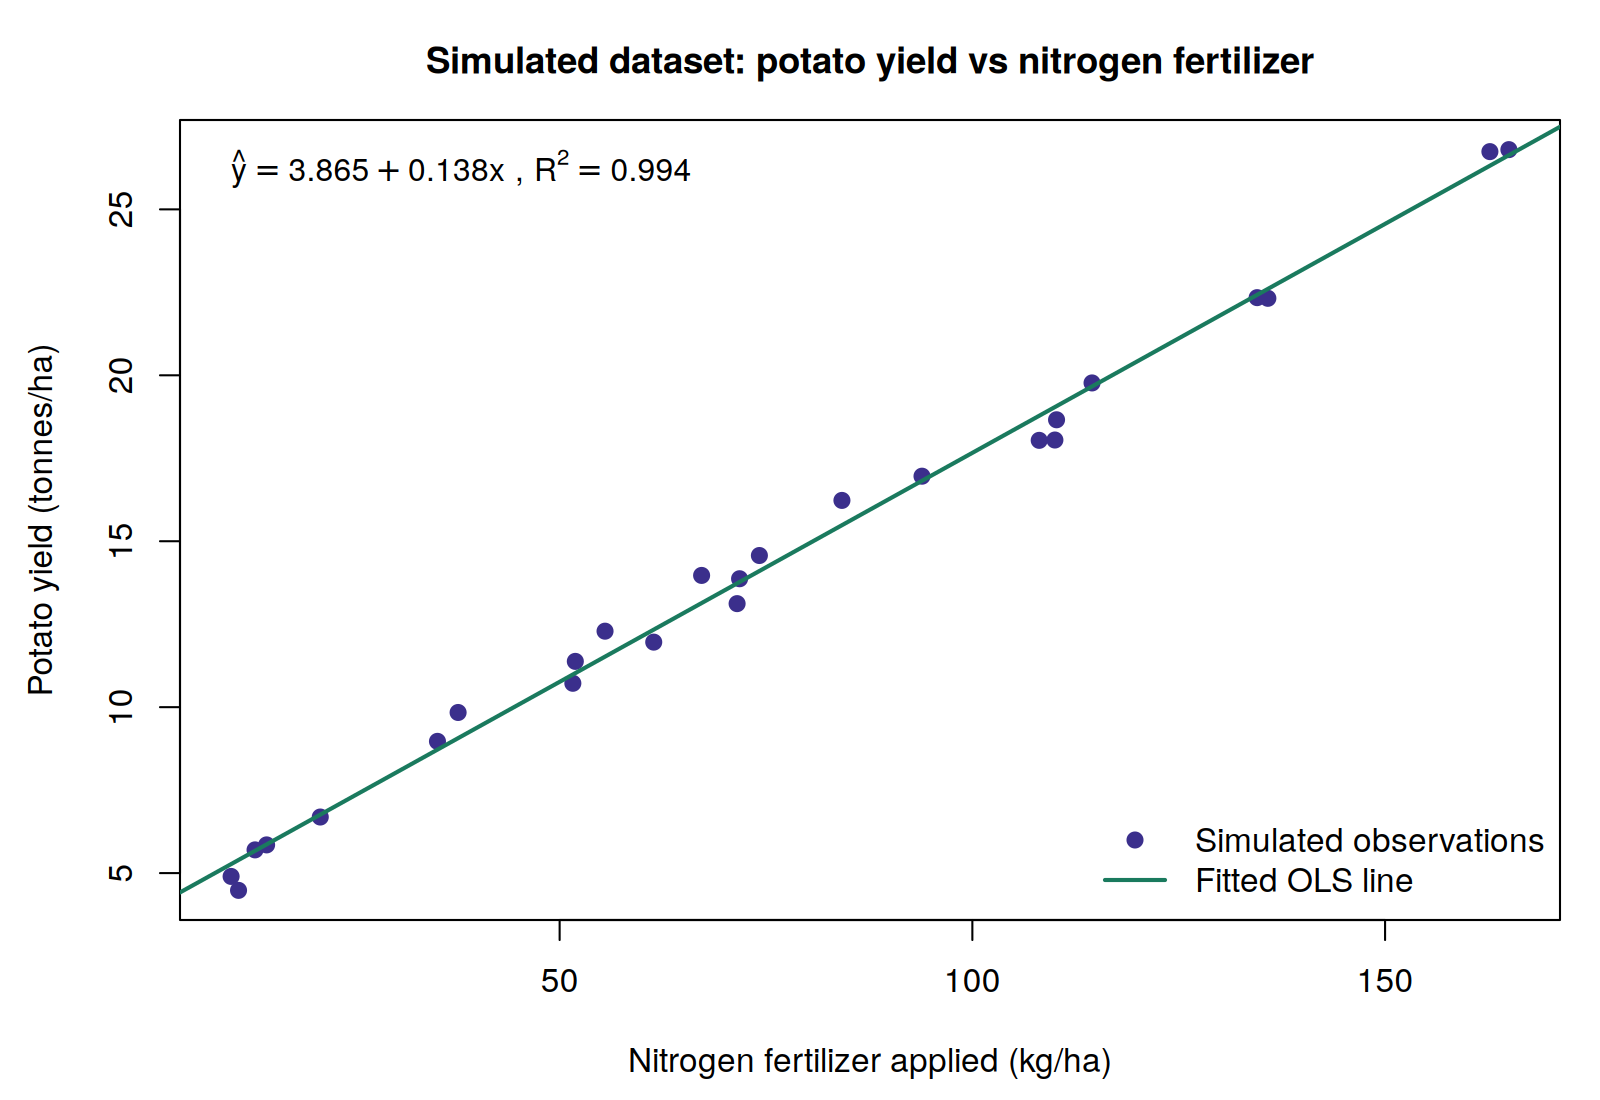
\includegraphics[width=0.85\linewidth]{assets/application-ols-simulation.png}
\end{screenshot}
\captionof{figure}{Simulated nitrogen-yield dataset with the fitted OLS line.}

The fitted line, $\hat y = 3.865+0.138x$ with $R^2=0.994$, lands almost exactly on the $\hat y = 3.94+0.139x$, $R^2=0.99$ seen in the exploration-phase figure, confirming that the by-hand normal equations, the matrix form $\hat\beta=(X^\top X)^{-1}X^\top Y$, and R's own \texttt{lm()} solver all converge on the same answer.


\chapter{Different Types of Response Variables}

\Exploration

To get a feel for this topic before formalising anything, I watched a video on different types of response variables on YouTube.

\begin{screenshot}
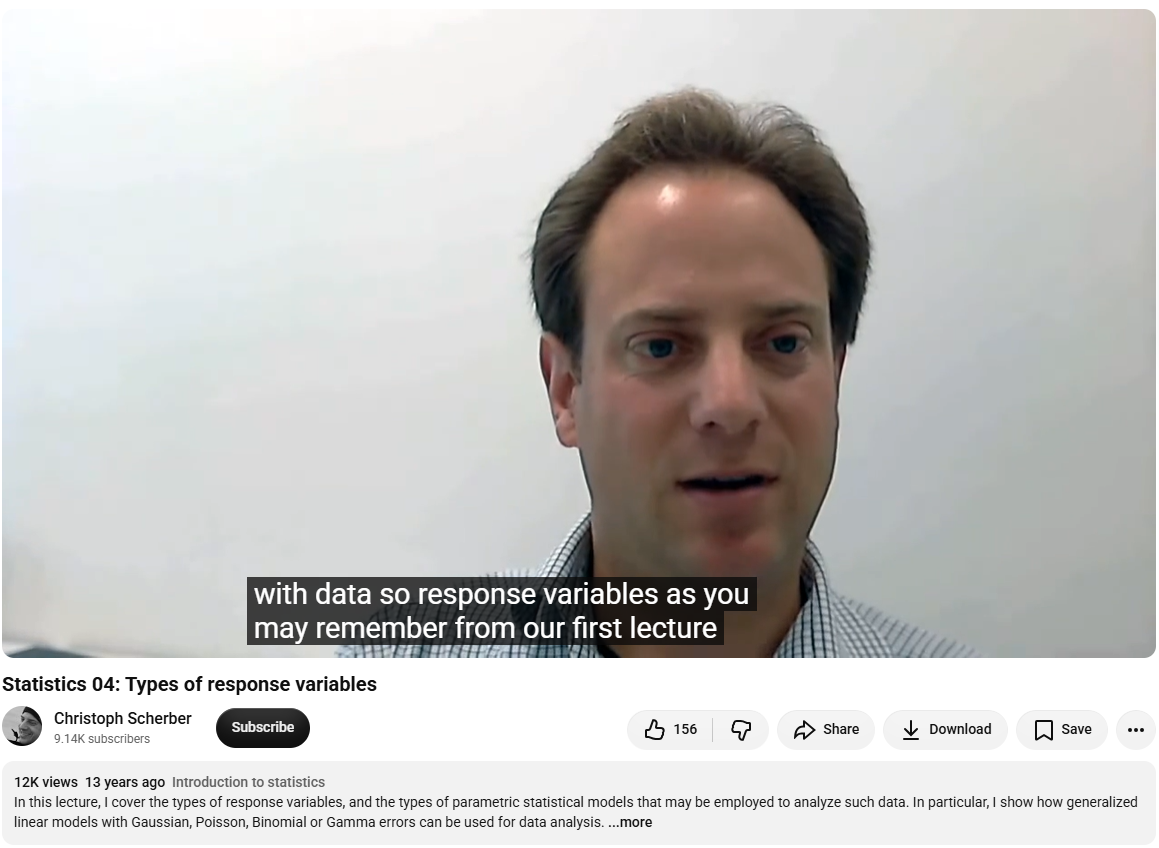
\includegraphics[width=\linewidth]{assets/exploration-response-variables-video.png}
\end{screenshot}
\captionof{figure}{Types of response variables, from a YouTube lecture \citep{scherber_response_variables}.}
\explorationsource{Scherber, C., \textit{Statistics 04: Types of Response Variables}, YouTube.}

From this video I picked up a few things about response variables:

\begin{enumerate}
\item A response variable is what we usually put on the $y$-axis, and it's dependent on the explanatory variables on the $x$-axis.
\item A response variable is the main output we're interested in, the main reason the model was built in the first place.
\item Since it's our aim, we can aim to do many different things with it: measure, count, partition. Because of this, we end up with different types of response variables, each carrying its own distribution.
\end{enumerate}

We move on to the Cognition phase, where these intuitions get sorted into a proper table.

\Cognition

Now, to build solid cognitive pillars on top of that intuitive background, the table below sets out the different response variables and the distributions that typically go with them.

\begin{table}[h]
\centering
\renewcommand{\arraystretch}{1.4}
\begin{tabular}{p{3.6cm}p{2.6cm}p{2cm}p{3.2cm}}
\toprule
\textbf{Outcome} & \textbf{Distribution} & \textbf{Typical Link} & \textbf{Form of $\eta$} \\
\midrule
Continuous, symmetric, can be positive or negative & Normal & Identity & $\mu$ \\
Binary (yes/no), proportion out of $n$ trials & Binomial (Bernoulli) & Logit & $\log\left(\dfrac{\pi}{1-\pi}\right)$ \\
Count, no fixed upper limit & Poisson & Log & $\log(\mu)$ \\
Count, overdispersed ($\operatorname{Var} \gg \operatorname{Mean}$) & Negative Binomial & Log & $\log(\mu)$ \\
Continuous, positive, right-skewed & Gamma & Log or Inverse & $\log(\mu)$ \\
\bottomrule
\end{tabular}
\caption{Common response variable types, their typical distributions, and typical link functions.}
\end{table}

$\eta$ is the same idea no matter which distribution is in play,
\begin{mathbox}
\[
\eta = \beta_0 + \beta_1 x_1 + \beta_2 x_2 + \cdots + \beta_k x_k
\]
\end{mathbox}
It's just the linear combination of explanatory variables. The link function is what connects $\eta$ to the mean of the outcome's distribution.

\begin{figure}[h]
\centering
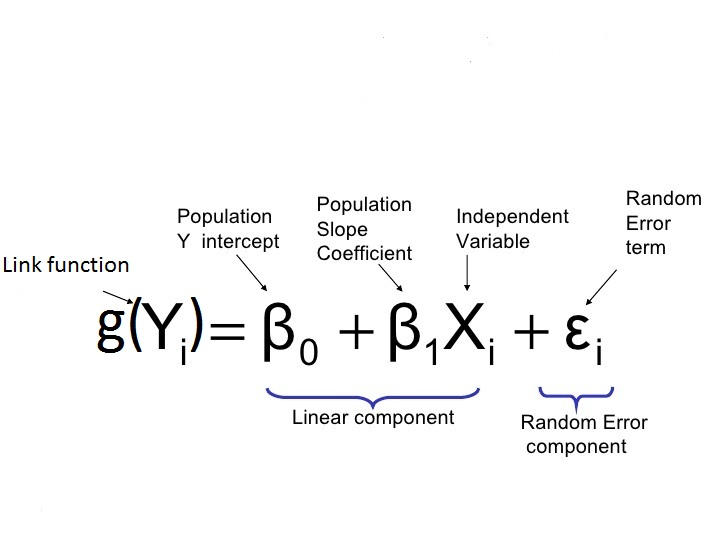
\includegraphics[width=0.7\linewidth]{assets/cognition-link-function-diagram.jpeg}
\caption{How a link function sits inside the linear predictor \citep{chandan_logistic}.}
\end{figure}

\Reflection

So, to reflect on this, let's work through a couple of scenarios and decide, each time, what distribution the response follows, then write out the linear component and link function to get some firsthand decision-making experience.

\subsection*{Scenario 1: Loan Default}
A bank wants to predict whether a customer defaults on a loan (yes/no), using annual income, credit score, and number of existing loans.

\begin{itemize}
\item \textbf{Outcome ($Y$):} Default (1 = yes, 0 = no).
\item \textbf{Explanatory ($X$'s):} Income, credit score, number of existing loans.
\item \textbf{Distribution:} Binomial (Bernoulli, one trial per customer).
\item \textbf{Link:} Logit.
\end{itemize}
\begin{mathbox}
\[
\eta = \beta_0 + \beta_1(\text{income}) + \beta_2(\text{credit score}) + \beta_3(\text{number of loans})
\]
\end{mathbox}

\subsection*{Scenario 2: Traffic Accidents}
\begin{itemize}
\item \textbf{Outcome ($Y$):} Number of accidents per month at an intersection (count, no natural cap).
\item \textbf{Explanatory ($X$'s):} Traffic volume, traffic light (yes/no), speed limit.
\item \textbf{Distribution:} Poisson.
\item \textbf{Link:} Log.
\end{itemize}
\begin{mathbox}
\[
\eta = \beta_0 + \beta_1(\text{traffic volume}) + \beta_2(\text{traffic light}) + \beta_3(\text{speed limit})
\]
\end{mathbox}

\begin{questionbox}[: Why do we bother with different types of response variables?]
As usual, to get at the real reason we generalise linear models, it helps to go back to why we make models at all: to get some outcome. In the simple linear model that outcome is usually just a continuous real number, typically unbounded except in special cases. But suppose we want to make inference on the proportion of rabbits with a certain deformity. Our outcome is now a binomial response, since each rabbit either has the deformity or doesn't, but what we actually want is the percentage of rabbits that get it. We still want to use a linear model to describe this, but for that to work we need to generalise the linear model using a link function, one that connects our binary outcomes to a linear predictor that gives back a continuous real number.
\end{questionbox}


\chapter{The Language of GLMs}

\Exploration

If GLMs were a demographic of people, they would have their own language. But to understand the language of these people, we first need to understand why we want to speak to them in the first place: what they eat, what they stand for, and their purpose in the grand scheme of things. Okay, enough of the analogy, before we dive into the boring definitions, let's take a moment to examine the actual aim of GLMs.

\textbf{Aim:} As simply as possible, the aim of GLMs is to know how a bunch of $X$'s affect a $Y$. That's the simplest definition.

Let's step into a time machine. This time machine takes us to 1972, when John Nelder and Robert Wedderburn formulated a framework for unifying various other statistical models, e.g.\ linear regression, logistic regression, and Poisson regression \citep{nelder1972}, along with a neat solution for maximum likelihood estimation known as the iteratively reweighted least squares method.

As we have already established intuitively, OLS predicts the expected value of a random variable $Y$ as a linear combination of a set of observed values (a ``bunch of $X$'s''), also known as predictors. We can make a few assumptions based on this:

\begin{enumerate}
\item A constant change in a predictor leads to a constant change in the response.
\item In the case of OLS, these assumptions hold when the response can vary indefinitely in both directions, i.e.\ it follows the pattern of a normal distribution.
\item However, when the response doesn't follow this pattern, we can use transformations to make it follow that pattern.
\item When these transformations are not sufficient, we employ the use of GLMs.
\end{enumerate}

\begin{screenshot}
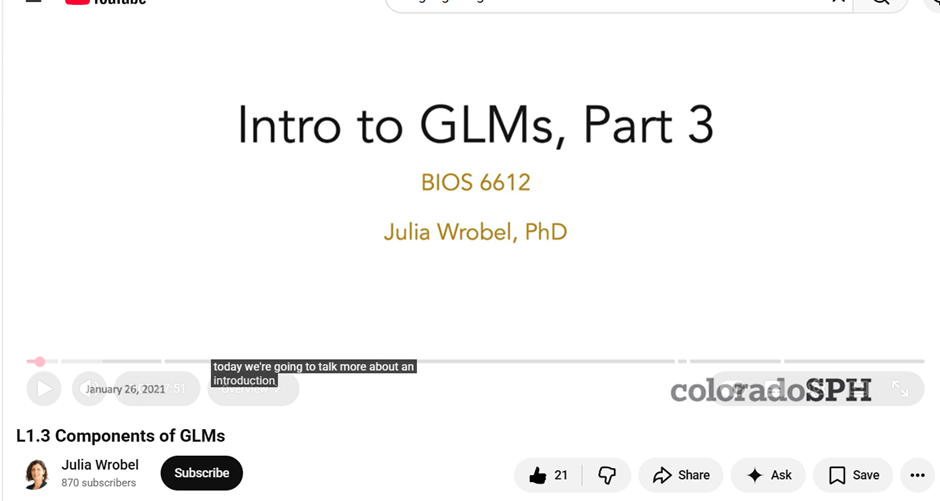
\includegraphics[width=0.75\linewidth]{assets/exploration-glm-components-video.png}
\end{screenshot}
\captionof{figure}{Components of GLMs, from a YouTube lecture \citep{wrobel_components}.}
\explorationsource{Wrobel, J. (2021, January 25), \textit{L1.3 Components of GLMs}, YouTube.}

Quick summary of this framework from a YouTube video I watched, before we dive into more definitions: assume that a known function of $\mu_i$ is related linearly to covariates,
\begin{mathbox}
\[
g(\mu_i) = \eta_i = x_i^\top\beta
\]
\end{mathbox}
Then:
\begin{enumerate}
\item $g$ = link function: links the linear predictor with the mean of the outcome.
\item We assume independence of $Y_i$.
\item The linearity assumption now applies to $\eta_i$, which need not equal $\mu_i$.
\item $X$ is treated as fixed.
\end{enumerate}

\Cognition

This chapter collects, in one place, the vocabulary used throughout the rest of the portfolio. Later chapters build on these terms without redefining them.

\term{Generalised Linear Model}
A generalised linear model is a generalisation of linear regression that is more versatile. The GLM generalises linear regression by connecting the linear model to the response variable via a link function, and by permitting the variance of each measurement to be a function of its predicted value \citep{nelder1972,mccullagh1989}.

\term{Log-linear Model}
A log-linear model is a mathematical model that allows for the application of potential multivariate linear regression by taking the form of a function whose logarithm equals a linear combination of the model's parameters:
\begin{mathbox}
\[
\exp\left\{c + \sum_i w_i f_i(X)\right\}
\]
\end{mathbox}
where $f_i(X)$ are functions of the vector of values $X$, and $c$ and $w_i$ are model parameters. Taking the natural log of this gives a linear combination that can be worked with directly \citep{agresti2015}.

\begin{defbox}[: Exponential Family]
An exponential family is a parametric set of probability distributions with the form
\[
f_X(x \mid \theta) = h(x)\exp\left\{\eta(\theta)\cdot T(x) - A(\theta)\right\}
\]
where $h(x)$ is non-negative and known, and $\eta(\theta)$, $T(x)$, $A(\theta)$ are known as well \citep{mccullagh1989,wikipedia_glm}.
\end{defbox}

\begin{defbox}[: One-Parameter Exponential Family]
A one-parameter exponential family is a special case of the exponential family in which the distribution depends on a single scalar parameter $\theta$, and its probability density (or mass) function can be written
\[
f(y;\theta) = \exp\left\{a(y)\,b(\theta) + c(\theta) + d(y)\right\}
\]
where $a(y)$ is the sufficient statistic, $b(\theta)$ is the natural (canonical) parameter, $c(\theta)$ is the log-partition function ensuring the density normalises to one, and $d(y)$ is the base measure, a term depending on $y$ alone. This form underlies several of the standard distributions used in GLMs, such as the Binomial and Poisson, for which the dispersion parameter is fixed at 1 \citep{taylor_nd}.
\end{defbox}

\term{Link Function}
A link function links the predicted mean of the response variable $\mu$ to the linear predictor $\eta$ in a GLM:
\begin{mathbox}
\[
g(\mu) = \eta = X\beta = \beta_0+\beta_1 x_1+\beta_2 x_2+\cdots+\beta_n x_n, \qquad \mu = g^{-1}(X\beta)
\]
\end{mathbox}
When $g$ is chosen such that the linear predictor equals the natural parameter of the distribution, it is called a canonical link function for that distribution, e.g.\ the logit link for the Binomial, or the log link for the Poisson \citep{dobson2018}.

\term{Transposed Matrix}
For any matrix $A$ with dimensions $m\times n$, the transpose $A^\top$ is the $n\times m$ matrix obtained by swapping its rows and columns: $(A^\top)_{ij} = A_{ji}$. Transposition is central to GLM estimation: for a design matrix $X$ and coefficient vector $\beta$, the normal equations used to estimate $\beta$ take the form $\hat\beta = (X^\top X)^{-1}X^\top y$, reflecting the orthogonality condition $X^\top(y-\mu(\beta))=0$ that arises from likelihood theory in GLMs \citep{casella2002}.

\term{Transposed Vector}
A transposed vector is a vector whose rows and columns have been flipped, so a column vector becomes a row vector or vice versa. For a column vector of covariates $x_i$ and column vector of coefficients $\beta$, $x_i^\top\beta = x_{i1}\beta_1+x_{i2}\beta_2+\cdots+x_{ip}\beta_p$, which is precisely the linear predictor $\eta_i$, a single scalar value \citep{casella2002}.

\term{Linear Predictor}
Denoted $X\beta$, this is the linear combination of covariates and regression coefficients that links the explanatory variables to the response distribution's mean through the link function \citep{dobson2018}.

\term{Parameters}
Quantities that characterise a probability distribution or a statistical model, whose values determine its shape, location, or scale. In a GLM, parameters include the regression coefficients ($\beta$), the dispersion parameter ($\phi$), and any other parameter implicit in the chosen distribution \citep{casella2002}.

\term{Sufficiency}
A property of a statistic whereby it captures all the information in a sample relevant to estimating a parameter, such that no other statistic calculated from the same sample provides additional information about that parameter \citep{casella2002}.

\term{Sufficient Statistic $a(y)$}
The statistic $a(y)$ that satisfies the property of sufficiency for a parameter. In exponential family notation, it is the function of the data multiplied by the natural parameter in the exponent. In many cases $a(y)=y$, and the distribution is then said to be in canonical form \citep[p.~2]{nowak_nd}.

\term{Natural Parameter $b(\theta)$}
Also called the canonical parameter, this is the parameter that appears in the exponent of a distribution written in exponential family form. It is the parameter through which the linear predictor connects to the distribution when a canonical link function is used \citep{mccullagh1989}.

\term{Log-partition Function $c(\theta)$}
Also called the cumulant function or normalising function, this ensures the exponential family density integrates (or sums) to one. Its derivatives generate the moments of the sufficient statistic: the first derivative gives the mean, the second gives the variance \citep{mccullagh1989}.

\term{Base Measure $d(y)$}
The component of the exponent that depends on $y$ alone, independent of $\theta$. It functions as a normalising term ensuring the density integrates to 1 \citep{mccullagh1989}.

\term{Dispersion Parameter}
A parameter, denoted $\phi$, that scales the variance of the response distribution independently of its mean. It reflects variability beyond what is explained by the mean-variance relationship of the chosen distribution. In the one-parameter exponential family form the dispersion parameter is fixed at 1 \citep{dobson2018}.

\term{Score Function}
The first derivative of the log-likelihood function with respect to the parameter(s) of interest. Setting the score function equal to zero and solving yields the maximum likelihood estimate \citep{casella2002}.

\term{Maximum Likelihood Estimates}
The parameter values that maximise the likelihood function, i.e.\ the values that make the observed data most probable under the assumed model. In GLMs, MLEs for $\beta$ are typically obtained via iterative methods such as Iteratively Reweighted Least Squares (IRLS), since closed-form solutions rarely exist outside the Gaussian case \citep{casella2002}.

\term{Canonical Form}
A distribution is said to be in canonical form when its sufficient statistic $a(y)$ equals $y$ itself, in which case the natural parameter is also called the canonical parameter \citep{mccullagh1989}.

\term{Logit}
The canonical link function for the binomial distribution, defined as the log-odds:
\begin{mathbox}
\[
g(\mu) = \log\left(\frac{\mu}{1-\mu}\right)
\]
\end{mathbox}
It maps probabilities bounded between 0 and 1 onto the entire real line, making it suitable for linear modelling \citep{dobson2018}.

\term{Probit}
A link function defined as the inverse of the standard normal cumulative distribution function, $g(\mu) = \Phi^{-1}(\mu)$. Commonly used for binary response models as an alternative to the logit link \citep{dobson2018}.

\term{Nuisance Parameter}
A parameter in a statistical model that is not of primary interest but must be accounted for in order to correctly estimate the parameters that are of interest. In many GLMs, the dispersion parameter is treated as a nuisance parameter \citep{casella2002}.

\Reflection
\tbc
